%!TEX TS-program = xelatex

% Шаблон документа LaTeX создан в 2018 году
% Алексеем Подчезерцевым
% В качестве исходных использованы шаблоны
% 	Данилом Фёдоровых (danil@fedorovykh.ru) 
%		https://www.writelatex.com/coursera/latex/5.2.2
%	LaTeX-шаблон для русской кандидатской диссертации и её автореферата.
%		https://github.com/AndreyAkinshin/Russian-Phd-LaTeX-Dissertation-Template

\documentclass[a4paper,14pt]{article}


%%% Работа с русским языком
\usepackage[english,russian]{babel}   %% загружает пакет многоязыковой вёрстки
\usepackage{fontspec}      %% подготавливает загрузку шрифтов Open Type, True Type и др.
\defaultfontfeatures{Ligatures={TeX},Renderer=Basic}  %% свойства шрифтов по умолчанию
\setmainfont[Ligatures={TeX,Historic}]{Times New Roman} %% задаёт основной шрифт документа
\setsansfont{Comic Sans MS}                    %% задаёт шрифт без засечек
\setmonofont{Courier New}
\usepackage{indentfirst}
\frenchspacing

\renewcommand{\epsilon}{\ensuremath{\varepsilon}}
\renewcommand{\phi}{\ensuremath{\varphi}}
\renewcommand{\kappa}{\ensuremath{\varkappa}}
\renewcommand{\le}{\ensuremath{\leqslant}}
\renewcommand{\leq}{\ensuremath{\leqslant}}
\renewcommand{\ge}{\ensuremath{\geqslant}}
\renewcommand{\geq}{\ensuremath{\geqslant}}
\renewcommand{\emptyset}{\varnothing}

%%% Дополнительная работа с математикой
\usepackage{amsmath,amsfonts,amssymb,amsthm,mathtools} % AMS
\usepackage{icomma} % "Умная" запятая: $0,2$ --- число, $0, 2$ --- перечисление

%% Номера формул
%\mathtoolsset{showonlyrefs=true} % Показывать номера только у тех формул, на которые есть \eqref{} в тексте.
%\usepackage{leqno} % Нумерация формул слева	

%% Перенос знаков в формулах (по Львовскому)
\newcommand*{\hm}[1]{#1\nobreak\discretionary{}
	{\hbox{$\mathsurround=0pt #1$}}{}}

%%% Работа с картинками
\usepackage{graphicx}  % Для вставки рисунков
\graphicspath{{images/}}  % папки с картинками
\setlength\fboxsep{3pt} % Отступ рамки \fbox{} от рисунка
\setlength\fboxrule{1pt} % Толщина линий рамки \fbox{}
\usepackage{wrapfig} % Обтекание рисунков текстом

%%% Работа с таблицами
\usepackage{array,tabularx,tabulary,booktabs} % Дополнительная работа с таблицами
\usepackage{longtable}  % Длинные таблицы
\usepackage{multirow} % Слияние строк в таблице
\usepackage{float}% http://ctan.org/pkg/float

%%% Программирование
\usepackage{etoolbox} % логические операторы


%%% Страница
\usepackage{extsizes} % Возможность сделать 14-й шрифт
\usepackage{geometry} % Простой способ задавать поля
\geometry{top=20mm}
\geometry{bottom=20mm}
\geometry{left=20mm}
\geometry{right=10mm}
%
%\usepackage{fancyhdr} % Колонтитулы
% 	\pagestyle{fancy}
%\renewcommand{\headrulewidth}{0pt}  % Толщина линейки, отчеркивающей верхний колонтитул
% 	\lfoot{Нижний левый}
% 	\rfoot{Нижний правый}
% 	\rhead{Верхний правый}
% 	\chead{Верхний в центре}
% 	\lhead{Верхний левый}
%	\cfoot{Нижний в центре} % По умолчанию здесь номер страницы

\usepackage{setspace} % Интерлиньяж
\onehalfspacing % Интерлиньяж 1.5
%\doublespacing % Интерлиньяж 2
%\singlespacing % Интерлиньяж 1

\usepackage{lastpage} % Узнать, сколько всего страниц в документе.

\usepackage{soul} % Модификаторы начертания

\usepackage{hyperref}
\usepackage[usenames,dvipsnames,svgnames,table,rgb]{xcolor}
\hypersetup{				% Гиперссылки
	unicode=true,           % русские буквы в раздела PDF
	pdftitle={ПРОЕКТИРОВАНИЕ И РАЗРАБОТКА ЭЛЕКТРОННОЙ СИСТЕМЫ ДЛЯ ДОПОЛНИТЕЛЬНОГО ОБРАЗОВАНИЯ СО ШКОЛЬНИКАМИ},   % Заголовок
	pdfauthor={Подчезерцев Алексей, Солодянкин Андрей},      % Автор
	pdfsubject={ПРОЕКТИРОВАНИЕ И РАЗРАБОТКА ЭЛЕКТРОННОЙ СИСТЕМЫ ДЛЯ ДОПОЛНИТЕЛЬНОГО ОБРАЗОВАНИЯ СО ШКОЛЬНИКАМИ},      % Тема
	pdfcreator={Подчезерцев Алексей, Солодянкин Андрей}, % Создатель
	pdfproducer={Подчезерцев Алексей, Солодянкин Андрей}, % Производитель
	pdfkeywords={МКР} {Moodle} {МИЭМ} {ВШЭ}, % Ключевые слова
	colorlinks=true,       	% false: ссылки в рамках; true: цветные ссылки
	linkcolor=black,          % внутренние ссылки
	citecolor=black,        % на библиографию
	filecolor=magenta,      % на файлы
	urlcolor=black           % на URL
}
\makeatletter 
\def\@biblabel#1{#1. } 
\makeatother
\usepackage{cite} % Работа с библиографией
%\usepackage[superscript]{cite} % Ссылки в верхних индексах
%\usepackage[nocompress]{cite} % 
\usepackage{csquotes} % Еще инструменты для ссылок

\usepackage{multicol} % Несколько колонок

\usepackage{tikz} % Работа с графикой
\usepackage{pgfplots}
\usepackage{pgfplotstable}

% ГОСТ заголовки
\usepackage[font=small]{caption}
%\captionsetup[table]{justification=centering, labelsep = newline} % Таблицы по правобу краю
%\captionsetup[figure]{justification=centering} % Картинки по центру


\newcommand{\tablecaption}[1]{\addtocounter{table}{1}\small \begin{flushright}\tablename \ \thetable\end{flushright}%	
\begin{center}#1\end{center}}

\newcommand{\imref}[1]{рис.~\ref{#1}}

\usepackage{multirow}
\usepackage{spreadtab}
\newcolumntype{K}[1]{@{}>{\centering\arraybackslash}p{#1cm}@{}}


\usepackage{xparse}
\ExplSyntaxOn
\DeclareExpandableDocumentCommand{\juliandate}{ m m m }
{
	\juliandate_calc:nnnn { #1 } { #2 } { #3 } { \use:n }
}
\NewDocumentCommand{\storejuliandate}{ s m m m m }
{
	\IfBooleanTF{#1}
	{
		\juliandate_calc:nnnn { #3 } { #4 } { #5 } { \cs_set:Npx #2 }
	}
	{
		\juliandate_calc:nnnn { #3 } { #4 } { #5 } { \cs_new:Npx #2 }
	}
}
\cs_new:Npn \juliandate_calc:nnnn #1 #2 #3 #4 % #1 = day, #2 = month, #3 = year, #4 = what to do
{
	#4 
	{
		\int_eval:n
		{
			#1 +
			\int_div_truncate:nn { 153 * (#2 + 12 * \int_div_truncate:nn { 14 - #2 } { 12 } - 3) + 2 } { 5 } +
			365 * (#3 + 4800 - \int_div_truncate:nn { 14 - #2 } { 12 } ) +
			\int_div_truncate:nn { #3 + 4800 - \int_div_truncate:nn { 14 - #2 } { 12 } } { 4 } -
			\int_div_truncate:nn { #3 + 4800 - \int_div_truncate:nn { 14 - #2 } { 12 } } { 100 } + 
			\int_div_truncate:nn { #3 + 4800 - \int_div_truncate:nn { 14 - #2 } { 12 } } { 400 } -
			32045
		}
	}
}

\tl_new:N \l__juliandate_g_tl
\tl_new:N \l__juliandate_dg_tl
\tl_new:N \l__juliandate_c_tl
\tl_new:N \l__juliandate_dc_tl
\tl_new:N \l__juliandate_b_tl
\tl_new:N \l__juliandate_db_tl
\tl_new:N \l__juliandate_a_tl
\tl_new:N \l__juliandate_da_tl
\tl_new:N \l__juliandate_y_tl
\tl_new:N \l__juliandate_m_tl
\tl_new:N \l__juliandate_d_tl
\int_new:N \l_juliandate_day_int
\int_new:N \l_juliandate_month_int
\int_new:N \l_juliandate_year_int

\cs_new:Npn \__juliandate_set:nn #1 #2
{
	\tl_set:cx { l__juliandate_#1_tl } { \int_eval:n { #2 } }
}
\cs_new:Npn \__juliandate_use:n #1
{
	\tl_use:c { l__juliandate_#1_tl }
}
\cs_new_protected:Npn \juliandate_reverse:n #1
{
	\__juliandate_set:nn { g }
	{ \int_div_truncate:nn { #1 + 32044 } { 146097 } }
	\__juliandate_set:nn { dg }
	{ \int_mod:nn { #1 + 32044 } { 146097 } }
	\__juliandate_set:nn { c }
	{ \int_div_truncate:nn { ( \int_div_truncate:nn { \__juliandate_use:n { dg } } { 36524 } + 1) * 3 } { 4 } }
	\__juliandate_set:nn { dc }
	{ \__juliandate_use:n { dg } - \__juliandate_use:n { c } * 36524 }
	\__juliandate_set:nn { b }
	{ \int_div_truncate:nn { \__juliandate_use:n { dc } } { 1461 } }
	\__juliandate_set:nn { db }
	{ \int_mod:nn { \__juliandate_use:n { dc } } { 1461 } }
	\__juliandate_set:nn { a }
	{ \int_div_truncate:nn { ( \int_div_truncate:nn { \__juliandate_use:n { db } } { 365 } + 1) * 3 } { 4 } }
	\__juliandate_set:nn { da }
	{ \__juliandate_use:n { db } - \__juliandate_use:n { a } * 365 }
	\__juliandate_set:nn { y }
	{
		\__juliandate_use:n { g } * 400 + 
		\__juliandate_use:n { c } * 100 + 
		\__juliandate_use:n { b } * 4 + 
		\__juliandate_use:n { a }
	}
	\__juliandate_set:nn { m }
	{ \int_div_truncate:nn { \__juliandate_use:n { da } * 5 + 308 } { 153 } - 2 }
	\__juliandate_set:nn { d }
	{ \__juliandate_use:n { da } - \int_div_truncate:nn { (\__juliandate_use:n { m } + 4) * 153 } { 5 } + 122 }
	\int_set:Nn \l_juliandate_year_int
	{ \__juliandate_use:n { y } - 4800 + \int_div_truncate:nn { \__juliandate_use:n { m } + 2 } { 12 } }
	\int_set:Nn \l_juliandate_month_int
	{ \int_mod:nn { \__juliandate_use:n { m } + 2 } { 12 } + 1 }
	\int_set:Nn \l_juliandate_day_int
	{ \__juliandate_use:n { d } + 1 }
}
\cs_generate_variant:Nn \juliandate_reverse:n { x }

\NewDocumentCommand{\showday}{ m }
{
	\juliandate_reverse:n { #1 }
	\int_to_arabic:n { \l_juliandate_day_int }-
	\int_to_arabic:n { \l_juliandate_month_int }-
	\int_to_arabic:n { \l_juliandate_year_int }
}

\NewDocumentCommand{\tomorrow}{ }
{
	\group_begin:
	\juliandate_reverse:x { \juliandate_calc:nnnn { \day + 1 } { \month } { \year } { \use:n } }
	\day = \l_juliandate_day_int
	\month = \l_juliandate_month_int
	\year = \l_juliandate_year_int
	\today
	\group_end:
}
\NewDocumentCommand{\tomorrowof}{ m m m }
{
	\group_begin:
	\juliandate_reverse:x { \juliandate_calc:nnnn { #1 + 1 } { #2 } { #3 } { \use:n } }
	\day = \l_juliandate_day_int
	\month = \l_juliandate_month_int
	\year = \l_juliandate_year_int
	\today
	\group_end:
}
\ExplSyntaxOff
\begin{document} % конец преамбулы, начало документа
\begin{titlepage}
	\begin{center}
		ФЕДЕРАЛЬНОЕ  ГОСУДАРСТВЕННОЕ АВТОНОМНОЕ \\
		ОБРАЗОВАТЕЛЬНОЕ УЧРЕЖДЕНИЕ ВЫСШЕГО ОБРАЗОВАНИЯ\\
		«НАЦИОНАЛЬНЫЙ ИССЛЕДОВАТЕЛЬСКИЙ УНИВЕРСИТЕТ\\
		«ВЫСШАЯ ШКОЛА ЭКОНОМИКИ»
	\end{center}
	
	\begin{center}
		\textbf{Московский институт электроники и математики}
		
		\textbf{Им. А.Н.Тихонова НИУ ВШЭ}
	\end{center}
	\vspace{1ex}	
	\begin{center}
		Солодянкин Андрей Александрович, группа БИВ172\\
		Подчезерцев Алексей Евгеньевич, группа БИВ172
	\end{center}	
	\vspace{1ex}
	\begin{center}
		\textbf{ТЕХНИЧЕСКОЕ ЗАДАНИЕ\\
		ПО МЕЖДИСЦИПЛИНАРНОЙ КУРСОВОЙ РАБОТЕ
	}
	\end{center}	
	\vspace{2ex}
	\begin{center}
		по теме «Проектирование и разработка электронной системы для дополнительного образования со школьниками»\\
	\end{center}
	\vspace{2ex}
	\begin{center}
%	Дата сдачи отчета: \today
	\end{center}
	\vspace{2ex}
	\vfill
	\begin{center}
		Москва \the\year г.
	\end{center}
\end{titlepage}

\section*{Аннотация}

%Количество страниц работы: \getlastpage, иллюстраций: \totalfigures, таблиц: \totaltables, источников: \LastBib.

\pagebreak

\section*{Annotation}

%Total number of pages is \getlastpage, figures: \totalfigures, tables: \totaltables, cite sources: \LastBib.
\pagebreak

\tableofcontents
\pagebreak

\section{Введение}

% Начало введения

% Актуальность
\subsection{Актуальность}

В настоящее время дополнительное образование получает все более широкое распространение.
Данный вид деятельности направлен на развитие внутренних и внешних качеств человека, укрепление личности, приобретении навыков работы в команде, изучении новых технологий и прочего развития.
Правительство принимает меры для продвижения данного вида образования [BIBER][https://rg.ru/2014/09/08/obrazovanie-site-dok.html], финансирование в данной сфере увеличивается.

Особенность дополнительного образования в том, что ученик сам выбирает интересующие направления, что должно улучшить качество процесса и повысить багаж знаний на выходе. 
 
% Новизна
\subsection{Новизна}

Особенность многих курсов -- разделение на только очные или только заочные. 
Первые иногда предоставляют доступ к своей системе, однако данные предназначены лишь для ознакомления с материалами лекций или семинаров, закрепления материала. 
У учеников нет возможности изучать что-то новое на базе платформы образовательной организации новую информацию.
Новизна нашего решения в том, что оно позволяет комбинировать очные встречи с преподавателями: координировать расписание, учитывать посещаемость; и дистанционные занятие: читать дополнительную литературу, проходить тестирование в любом месте на одной и той же платформе.

% Объект
\subsection{Объект исследования}

Исходя из вышесказанного, объект исследования -- существующие платформы дополнительного образования, фреймворки и среды для создания таких платформ.
Необходимо изучить свойства каждого решения и возможность доработки для создания универсальной подходящей платформы.

% Предмет

% Цель
\subsection{Цель работы}
Таким образом, цель данной работы -- получение электронной системы для обеспечения электронной образовательной среды проекта по дополнительному образованию школьников в МИЭМ НИУ ВШЭ.

% Задачи
\subsection{Задачи работы}
Для достижения данной цели были поставлены следующие задачи:
\begin{itemize}
	\item Изучить существующие решения в области дополнительного образования;
	\item Разработать собственную платформу на базе одной из существующих;
	\item Интегрировать систему с ресурсами НИУ ВШЭ;
	\item Произвести тестирование системы.
\end{itemize}

% Значимость
\subsection{Практическая значимость}
После создания данной системы появится возможность автоматизировать однотипные и рутинные действия в существующей системе дополнительного образования.
Кроме того, школьники получат возможность закрепить, повторить и изучить дополнительную информацию дома после учёбы на курсах.
Преподаватели получат систему для организации курсов и контролю процесса.

% Личный вклад

% Конец введения

\pagebreak

% ==============================================================================
% Начало Г1

\section{Обзор и анализ предметной области}

% Comment - надо аккуратно перенести часть текста во 2 главу, чтобы GIT не ругался

\subsection{Состояние предметной области}

Важной частью современного образования является дополнительные образовательные программы, которые направлены на разностороннее развитие личных качеств.
Секции, кружки по интересам, образовательные курсы получили широкое распространение во многих странах мира.
Некоторые учебные программы финансируются государством, другие привлекают школьников или студентов для дальнейшей учёбы или работы.

Современный курс может носить как дистанционный, так и очный характер, однако в любом случае необходимо организовать данный процесс.
Преподавателям и руководителям требуется контролировать запись и посещаемость, распространение справочного материала, проводить срез знаний, проверять работы, вести учёт оценок и выполнять множество других однотипных действий.
Логичным решением данной проблемы есть автоматизация данного процесса с использованием программных средств.

Данный подход широко используется в современном образовании. В частности, многие организации используют собственные системы контроля образовательного процесса или подключаются к уже готовым решениям.

\subsection{Описание подобных решений}

В настоящее время на рынке существует огромное количество систем дистанционного обучения. Среди них можно выделить такие платформы, как:
\begin{itemize}
	\item Coursera
	\item Stepic
	\item Открытое образование (openedu)
	\item LMS HSE
\end{itemize}

\textbf{Coursera}

Одна из самых популярных образовательных платформ, созданная профессорами Стэнфордского университета Эндрю Ыном и Дафной Коллер. 

Система содержит в себе курсы от ведущих мировых вузов, это является одновремнно положительной и отрицательной чертой. С одной стороны, обучающиеся получают  очень качественную и проверенную информацию. С другой стороны, далеко не каждый человек может создать курс.

В системе не предусмотрено очное посещение курсов, а следовательно не составляется расписание очных занятий.

Доступ к материалам курсов можно получить через сайт и через специальные приложения для iOS и Android.

\textbf{Stepic}

Российская образовательная программа, разработанная Николаем Вяххиным. Позволяет создавать обучающие уроки и онлайн-курсы всем зарегистрированным пользователям. Для проверки используются разнообразные задачи с автоматической проверкой и моментальной обратной связью.

Отдельные элементы платформы Stepic используются для проверки заданий в других образовательных системмах.

В этой системе тоже не предуссмотрено очное посещение, значит и срасписания очных занятий, и учета посещаемости не будет.

Помимо сайта существуют версии приложения для iOS и Android.

\textbf{Открытое образование (openedu)}

Образовательная платформа, предлагающая российским университетам размещать свои курсы. Основана ведущими российскими вузами - МГУ им. М.В. Ломоносова , СПбПУ, СПбГУ, НИТУ «МИСиС», НИУ ВШЭ, МФТИ, УрФУ и Университет ИТМО.

Данная платформа для дополнителного образования создана на основе системы open edX.

\textbf{LMS HSE}

LMS HSE (система управления обучением) созданна в НИУ ВШЭ на основе системы eFront. Пердоставляет доступ к учебным материалам курсов, возможность загрузки домашнего задания, содержит в себе различную информацию касательно образовательного процесса, помогает поддерживать связь между преподавателями и студентами.
Помимо всего этого образовательная система помогает организовать и внеучебные мероприятия. 

Из недостатков LMS HSE можно выделить то, что в этой системе отсутствует возможность автоматической проверки выполненных заланий.


% Г1 - детальное и подробное описание существующих технологий

% Г1 - детальное и подробное описание аналогичных технологических решений

% Г1 - анализ технологий

% Г1 - Выбор Решения - таблица сравнения
\begin{table}[H]
	\begin{tabular}{|l|l|l|l|l|l|}
		\hline
		& Coursera & Stepic & openedu & LMS HSE & наше приложение \\ \hline
		расписание занятий & - & - & - & ± & + \\ \hline
		\begin{tabular}[c]{@{}l@{}}электронный журнал \\ учета посещаемости\end{tabular} & - & - & - & - & + \\ \hline
		online тестирование & + & + & + & - & + \\ \hline
		\begin{tabular}[c]{@{}l@{}}автоматизированная\\  проверка \\ программного кода\end{tabular} & ± & + & ± & - & + \\ \hline
		\begin{tabular}[c]{@{}l@{}}осуществление \\ массовых рассылок\end{tabular} & + & + & + & + & + \\ \hline
		доступность??? & - & + & - & ± & + \\ \hline
	\end{tabular}
\end{table}

\subsection{Выводы и заключение}

В данной главе были рассмотрены аналоги, их достоинства и недостатки, ни один из рассмотренных аналогов не сочетает все каства для удобства проведения очных занятий и дистанционного обучения. Отсюда выдвигаются требования к нашему приложению:

\begin{itemize}
	\item Составление и отображение расписания занятий
	\item Электронный журнал учета посещвемости
	\item online тестирование
	\item автоматизированная проверка программного кода
	\item Осуществление массовых рассылок

\end{itemize}

% Г1 - Выводы и заключение


% Конец Г1
% ==============================================================================
% Начало Г2

% Методы решения

\section{Обзор и анализ методов решения}

В данный момент существует большое количество систем для организации онлайн курсов.
Каждая из них отличается интерфейсом, системой управления и администрирования, возможностью модернизации и другими параметрами.

\subsection{Анализ существующих решений}

Для сравнения были выбраны следующие наиболее популярные системы:

\begin{itemize}
	\item iSpring Online LMS
	\item Moodle	
	\item Open edx
	\item LMS HSE
\end{itemize}

Опишем каждую из них.

\subsubsection{iSpring Online LMS}

Данная система относится к проприетарным решениям с закрытым исходным кодом.
С одной стороны, разработчики заинтересованы в создании качественного и удобного решения для конечного пользователя, но с другой стороны такое решение будет требовать дополнительных ежемесячных затрат на пользование системой.[BIBER][тот же сайт этой фигни]
Аналогов iSpring Online LMS существует много, их объединяет одно -- платный доступ, закрытый код и наличие технической поддержки.
Их объединяет следующие преимущества этих систем: простота в установке и управлении
К основными чертам таких систем можно отнести:
\begin{itemize}
	\item простота в установке;
	\item простота в управлении;	
	\item профессиональная техническая поддержка.
\end{itemize}

При этом у них присутствуют следующие недостатки:
\begin{itemize}
	\item отсутствие кастомизации
	\item стоимость системы
\end{itemize} 

\subsubsection{LMS eFront}

% http://blog.uchu.pro/lms-efront/ 
% https://en.wikipedia.org/wiki/EFront_(eLearning_software)
Данный фреймворк используется в НИУ ВШЭ [BIBER][11 04 2019], ранние версии распространялись под свободной лицензией CPAL [BIBER], однако сейчас на официальном сайте предлагаются коммерческие решения.
Из достоинств системы можно выделить:

\begin{itemize}
	\item Чёткая вёрстка веб-страниц, стабильная работа программной оболочки;
	\item Подробные отчёты о деятельности пользователей с гибкой фильтрацией.	
\end{itemize} 

Недостатки системы:

\begin{itemize}
	\item Относительно небольшое количество инструментов для создания учебных материалов;
	\item Относительно мало дополнительных модулей;
	\item Малое сообщество пользователей.
\end{itemize} 

\subsubsection{Moodle}

Moodle - крупнейшая и самая популярная система управления курсами, которая активно развивается с 2002 года.
Важными преимуществами этой системы являются:

\begin{itemize}
	\item Бесплатность системы;
	\item Неограненный возможности кастомизации;
	\item Наличие широкого функционала для обеспечения процесса обучения (есть почти всё);
	\item Бесплатная, с открытым исходным кодом;
	\item Большое онлайн-сообщество на официальном сайте.
\end{itemize} 

Минусы системы:

\begin{itemize}
	\item Сложна для освоения;
\end{itemize} 


\subsubsection{Open edX} 

Платформа Open edX была создана Массачусетским технологическим институтом совместно с Гарвардским университетом[BIBER][WIKI].
Данная платформа позволяет создавать массовые онлайн курсы, ориентированные для широкой аудитории.

К достоинствам данного решения можно отнести:

\begin{itemize}
	\item Открытый исходный код платформы;
	\item Разнообразие плагинов для расширения функционала;
	\item Большое сообщество разработчиков;
\end{itemize}

Недостатки:

\begin{itemize}
	\item Система ориентирована на массовое дистанционное обучение;
	\item Сложность с интеграцией с существующими проектами образовательного учреждения;
\end{itemize}

\subsubsection{Собственное решение} 

\textbf{Написать решение с <<Нуля>>} часто рассматривается при проектировании.
Оно позволит создать продукт с функционалом, наиболее подходящим к желанию заказчика.

Достоинства подхода:

\begin{itemize}
	\item Возможность создать продукт с максимальным соответствием требованиям;
	\item Отсутствие зависимостей от сторонних готовых CMS.
\end{itemize}

Однако, данный подход содержит существенный недостаток: высокая стоимость разработки (в человеко-часах).
Разработчикам придётся создать весь функционал, который существует в готовых решениях,  и ещё добавить связанный с конкретной задачей.
Кроме того, не будет достаточно времени и ресурсов для полного тестирования системы.

% Анализ методов

% TODO совпадение с предыдущим пунктом?

% Выбор метода

\subsection{Выбор метода решения}

\begin{landscape}
	\begin{table}[!h]
		\begin{center}
			\begin{flushleft}
				\tablecaption{Сравнение основных систем}
			\end{flushleft}
			
			\begin{tabular}{|l|l|l|l|l|l|}
				\hline
				& iSpring Online LMS & LMS eFront & Moodle & Open edX & Собственное решение \\ \hline
				Бесплатно                              & -                  & +          & +      & +        & +                   \\ \hline
				Малое время разработки                 & +                  & +          & +      & +        & -                   \\ \hline
				Наличие широкого сообщества            & техподдержка       & ±          & +      & +        & -                   \\ \hline
				Возможность кастомизации               & -                  & ±          & ±      & ±        & +                   \\ \hline
				Простота разработки                    & -                  & ±          & +      & +        & -                   \\ \hline
				Простота обслуживания                  & +                  & ±          & ±      & ±        & +                   \\ \hline
				Надежность                             & +                  & +          & +      & +        & -                   \\ \hline
				Ориентация на традиционное образование & +                  & +          & +      & -        & +                   \\ \hline
			\end{tabular}
		\end{center}
	\end{table}
\end{landscape}

На основании вышесказанного, для разработки была выбрана система Moodle как наиболее полно удовлетворяющая требованиям к проекту.

\subsection{Выводы по главе}

За основу была взят последний стабильный релиз Moodle на Github, в качестве сервера баз данных -- MySql последней версии(требование заказчика), последняя стабильная версия PHP 7.3, разработка велась на операционной системе Windows 10, деплой и тестирование в Ubuntu 16.04 на VPS. 
Кроме того, были рассмотрены существующие CMS для создания платформ курсов, оценены их достоинства и недостатки.

% Заключение и выводы

% Конец Г2
% ==============================================================================
% Начало Г3
\section{Теоретические основы системы} 

Основное отличие нашего решения от всевозможных модернизаций Moodle -- наличие интеграции с серверами НИУ ВШЭ для автоматического управления расписанием.
Необходимо разработать структуру хранения, получения, обработки и вывода информации о занятиях.

\subsection{Проектирование баз данных}

Новая система должна хранить расписание занятий для ускорения обработки данных.
Кроме того, каждый курс должен знать информацию о номере группы в РУЗе для получения обновлений.
На первый взгляд, логичным решением будет добавление дополнительного атрибута в таблицу курса, который будет указывать на номер группы, однако такое решение может повлиять на внутреннюю работу системы Moodle, поэтому было решено создать дополнительную таблицу со связью 1 к 1 с таблицей курса.
Дополнительно была создана таблица для хранения кэшей расписание, содержащая основные атрибуты, возвращаемые сервисом расписания, и номер группы, к которой относится конкретное занятий (Рис. \ref{img:db_struct}).

\begin{figure}[H]
	\centering		
	\includegraphics[width=\linewidth]{schemas/database}
	\caption{Схема базы данных}\label{img:db_struct}
\end{figure}

\subsection{Проектирование классов и методов}

Для удобства обращения к другим WEB ресурсам была создана обёртка над стандартной программой cURL, предназначенной для отправки запросов на другие сервера (Рис. \ref{img:request_class}).
Итоговый вариант в конструкторе устанавливал параметры для отправки запроса и, в случае успеха ответа, приводил ответ из JSON формата в структуры PHP.
После окончания работы с запросом соединение автоматически закрывалось.

\begin{figure}[H]
	\centering		
	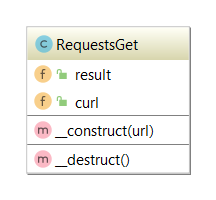
\includegraphics{image/RequestsGet}
	\caption{Структура класса RequestsGet}\label{img:request_class}
\end{figure}

Более важным в проекте является класс для работы с базой данных курса (Рис. \ref{img:db_class}). 
Данная структура агрегирует различные методы для создания, изменения и удаления сущностей.
Объект был создан с применением паттерна Singleton, так как сам класс не хранит данные, а лишь обращается к базе данных.
При первом создании экземпляра проверяется наличие необходимых таблиц, в случае их отсутствия они будут автоматически созданы.
Простые запросы реализованы с помощью Moodle ORM для сокращения кода, более сложные со множеством условий и соединением таблиц написаны вручную.


\begin{figure}[H]
	\centering		
	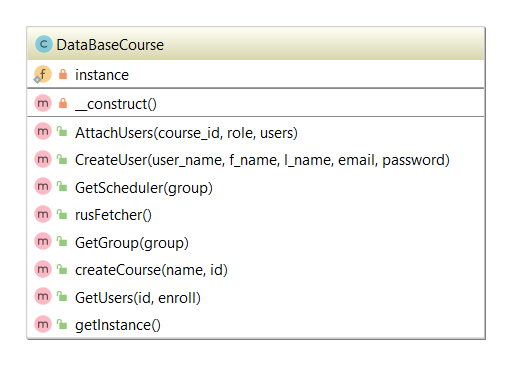
\includegraphics[width=0.7\linewidth]{image/DataBaseClass}
	\caption{Структура класса DataBaseCourse}\label{img:db_class}
\end{figure}

\subsection{Проектирование пользовательского интерфейса}

После установки и знакомством с пользовательским интерфесом администратора были обнаружены его недостатки: перегруженность и сложность для нового пользователя.
Переходы между разделами бывают не совсем логичными или доступны при установке дополнительных параметров на специальных страницах.
Было решено спроектировать отдельную страницу для управления администратором связями с данными расписания и выполнением базовых действий с существующими, новыми и будущими пользователями.
Логика переходов отражена на Рис. \ref{img:UI}.

\begin{figure}[H]
	\centering		
	\includegraphics[width=\linewidth]{schemas/UI}
	\caption{Схема переходов в пользовательском интерфейсе}\label{img:UI}
\end{figure}

В центре синим цветом изображены страницы, непосредственно с которых происходит взаимодействия пользователя.
Стрелками показаны возможные переходы между страницами и действия на них.
Красными выделены блоки, которые являются частью интерфейса Moodle.

% Модели

% Методы

% Алгоритмы

% Схемы

% UML

% Выводы
\subsection{Выводы по главе}

В данной части были рассмотрены ключевые элементы проектирования, а именно схема отношений баз данных, структура классов и их функционал, схема взаимодействия администратора с интерфейсом управления курсом.

% Конец Г3
% ==============================================================================
% Начало Г4

\section{Практическая реализация}
% Описание решения
\subsection{Подготовка окружения}

Для разработки была взята последняя стабильная версия 3.6.1 на GitHub, однако история разработки была сброшена, так как проект Moodle имеет слишком большую историю разработки и более 90 тысяч коммитов только в главной ветке.
Для хостинга кода был создан приватный репозиторий на GitHub.

В качестве сервера был использован уже имеющийся хостинг VPS DigitalOcean с сервером в Лондоне на минимальном тарифном плане (1 vCPU, 1 ГБ RAM, 25 ГБ SSD), на котором были уже установлены СУБД MySQL и web сервер NGINX для других проектов.
Было выделено доменное имя 3 уровня \url{lms.asciishell.site} на собственном домене.
Был создан новый unix пользователь для работы с новым сервисом, настроен доступ к репозиторию по ключу.
Кроме того, для успешной работы Moodle понадобилось установить php интерпретатор и apache. 
После потребовалось настроить NGINX прокси и apache для совместной работы, сконфигурировать LetsEncrypt для выдачи и автоматического обновления сертификата безопасности сайта.
Для разработки был использован Open Server с MySQL и php.
На данном этапе первичная настройка была окончена, чего было достаточно для разработки и тестирования на реальном сервере.

\subsection{Установка плагинов}

Многий функционал в Moodle добавляется и настраивается с помощью специальных пакетов -- плагинов -- которые расширяют функционал приложения.
Moodle имеет богатую библиотеку плагинов, позволяющие решить практически любую типовую задачу.

В первую очередь был установлен и настроен \textbf{CodeRunner} и зависимые плагины.
Данный плагин позволяет создавать вопросы с проверкой программного кода ученика на многих языках, в том числе на Python, C++ и JavaScript.

Для большего удобства дальнейшей работы были установлены расширения для подсветки исходного кода для повышения удобочитаемости и привитию привычки к качественному коду у учеников.

Кроме того, были добавлены плагины с вопросами на упорядочивание данных и соотношения для увеличения возможностей преподавательского состава проверять знания учащихся.

\subsection{Настройка почты}

Одна из функций нашей платформы -- рассылка почты.
Данный функционал присутствует практически в каждом современном сайте с регистрацией пользователя.
С помощью почты пользователь может получать уведомления от учителя, администратора, взаимодействовать с другими пользователями.

В качестве сервера почты был выбран Яндекс.Коннект, который предоставляет удобный и понятный интерфейс для управления записями доменного имени, а так же не менее простой и бесплатный сервис по настройке почты для своего домена (Рис. \ref{img:yandex}).
Был создан почтовый ящик, с которого необходимо производить рассылку корреспонденции (Рис. \ref{img:miemMail}), далее установлен и настроен почтовый сервер postfix для приёма писем с Moodle и пересылкой их на сервера Яндекса.
В Moodle сервером получателем был указан localhost.

\begin{figure}[H]
	\centering
	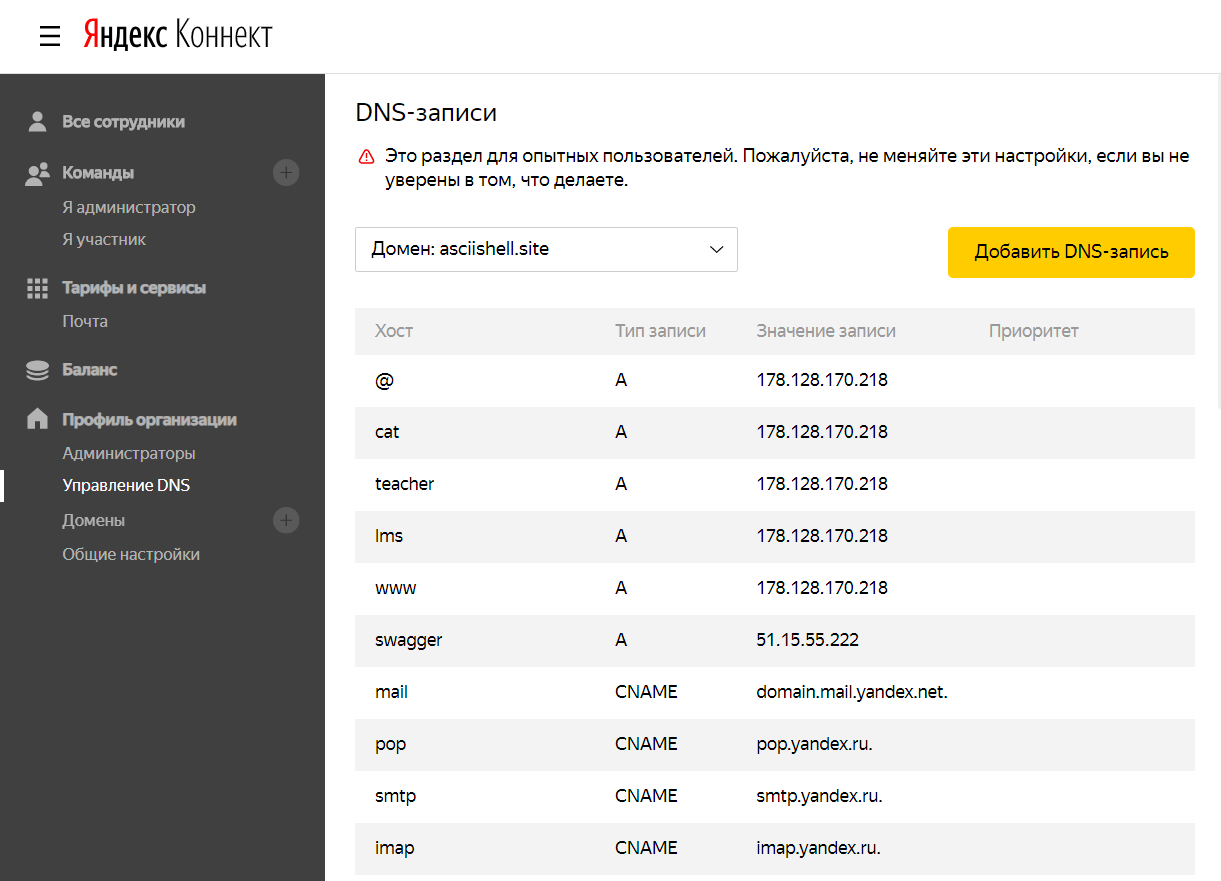
\includegraphics[width=0.7\linewidth]{image/yandex_connect}
	\caption{Интерфейс администратора домена Яндекс.Коннект}
	\label{img:yandex}
\end{figure}

\begin{figure}[H]
	\centering
	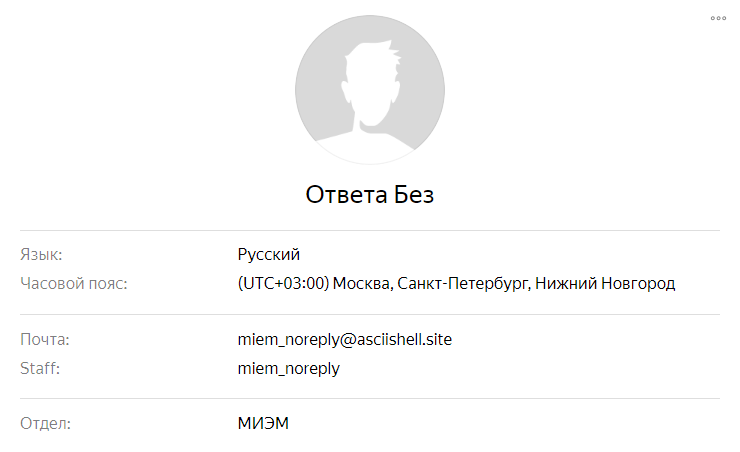
\includegraphics[width=0.7\linewidth]{image/yandex_miem}
	\caption{Учётная запись почтовой рассылки}
	\label{img:miemMail}
\end{figure}

\subsection{Интеграция с РУЗом}

Одна из самых ресурсозатратных задач данной работы -- интегрировать взаимодействие с сервером расписаний учебных занятий для реализации поиска по группе и автоматического обновления расписания.
Был произведён анализ трафика на странице \url[РУЗа]{https://ruz.hse.ru/ruz/main}, где была выявлена схема взаимодействия с backend-ом.
Полученные данные были использованы для составления собственных запросов.
Сервер возвращал информацию в формате JSON, поэтому не возникло трудностей с обработкой результата.
Были созданы таблицы, реализованы методы для работы с базой данных и отправкой запросов на удалённый сервер.
Кроме того, были свёрстаны страницы для красивого и удобного пользовательского интерфейса.

% Описание экспериментов

% Демонстрация
\subsection{Демонстрация работы}

Дополнительный интерфейс размещён по адресу \url{/ruz}, который разрешает доступ только авторизованным пользователям с правами администратора, в противном случае пользователю откажут в доступе (Рис. \ref{img:ui_login}).
	
\begin{figure}[H]
	\centering
	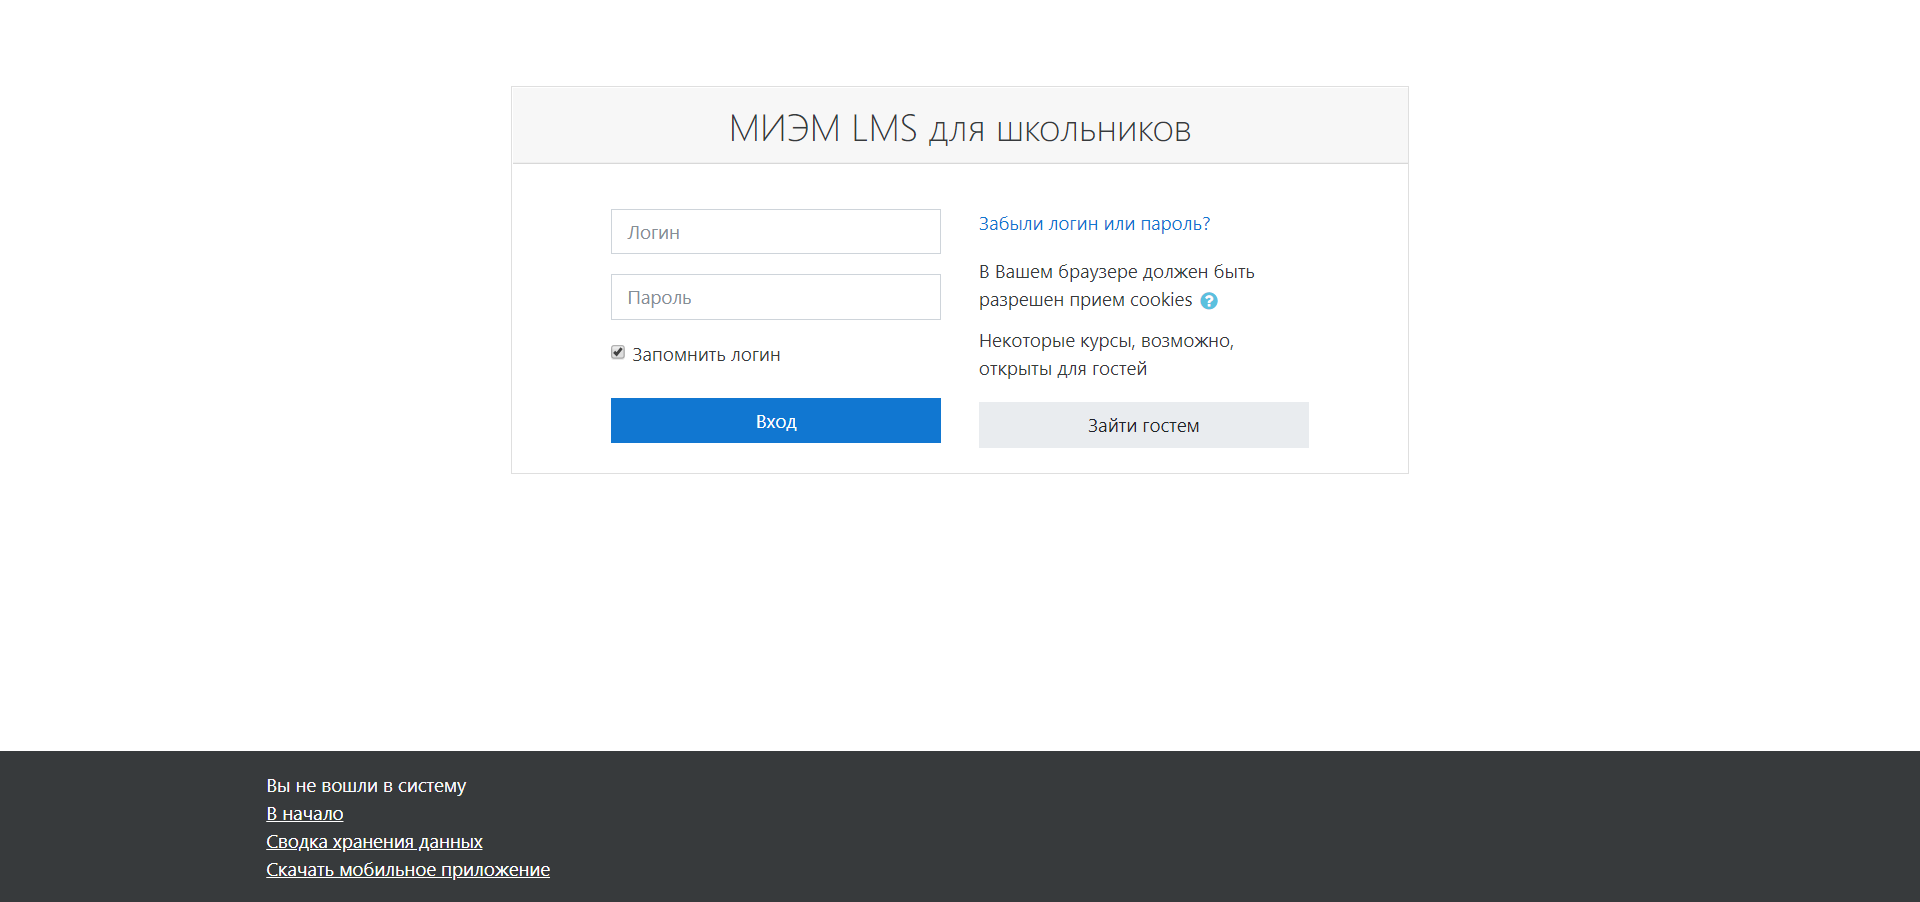
\includegraphics[width=\linewidth]{image/ui_login}
	\caption{Страница входа}
	\label{img:ui_login}
\end{figure}

В случае успешной авторизации пользователь попадает в панель администратора, на главной странице которой выведен список всех групп (Рис. \ref{img:ui_listOfGroups}).
На данной странице можно перейти непосредственно к курсу, посмотреть его номер в РУЗе, записать пользователей с интересующей ролью (Рис. \ref{img:ui_enroll}), посмотреть расписание данной группы (Рис. \ref{img:ui_scheduler}) или перейти к редактированию.

\begin{figure}[H]
	\centering
	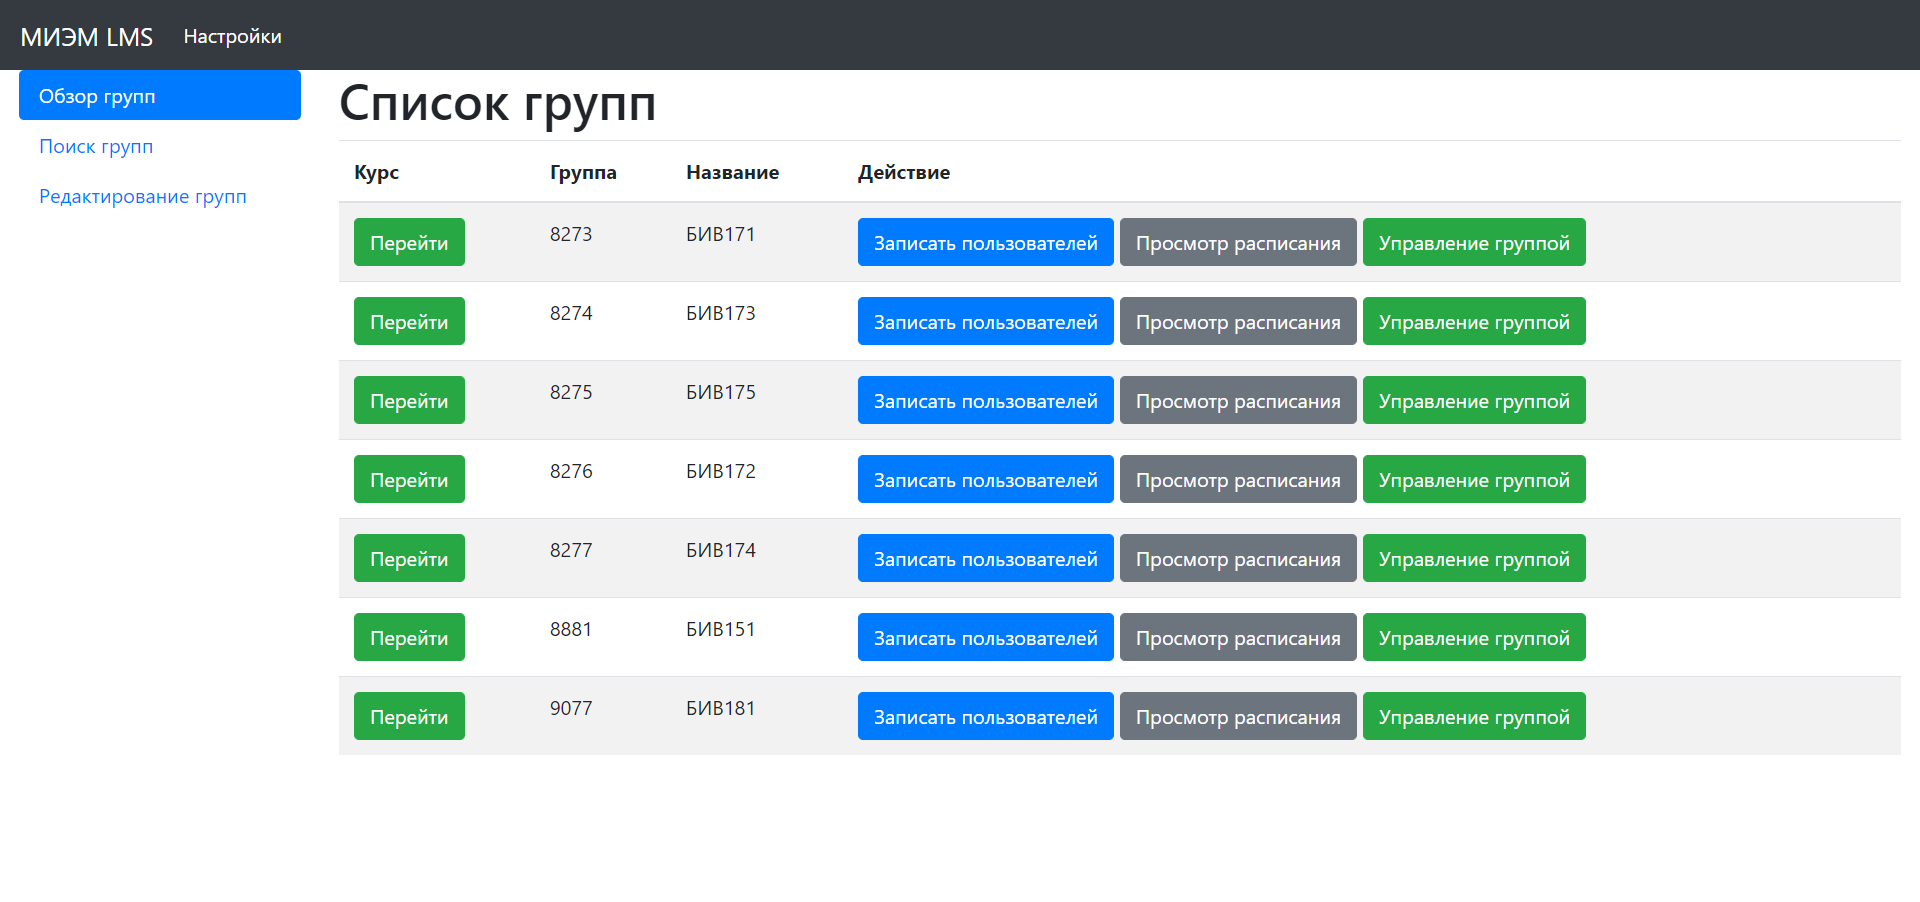
\includegraphics[width=\linewidth]{image/ui_listOfGroups}
	\caption{Главная страница -- обзор групп}
	\label{img:ui_listOfGroups}
\end{figure}

\begin{figure}[H]
	\centering
	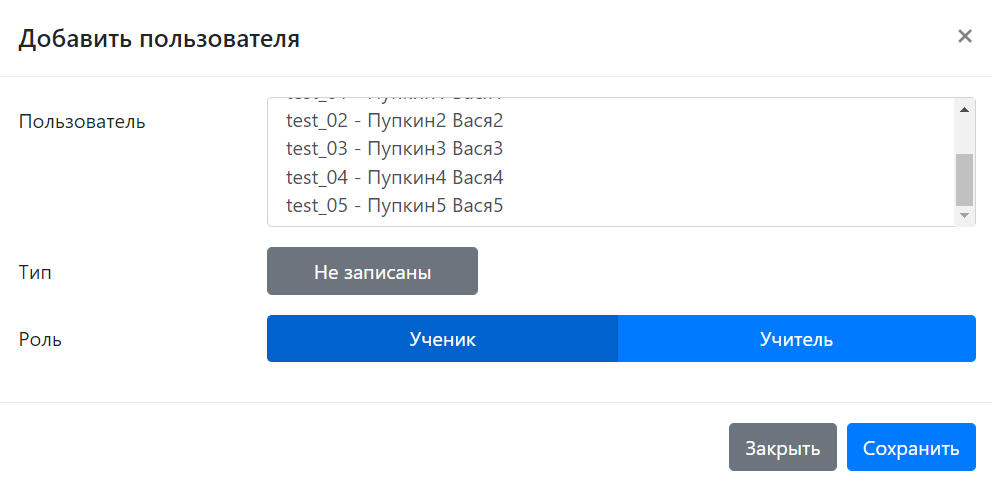
\includegraphics[width=\linewidth]{image/ui_enroll}
	\caption{Форма записи на курс}
	\label{img:ui_enroll}
\end{figure}
\begin{figure}[H]
	\centering
	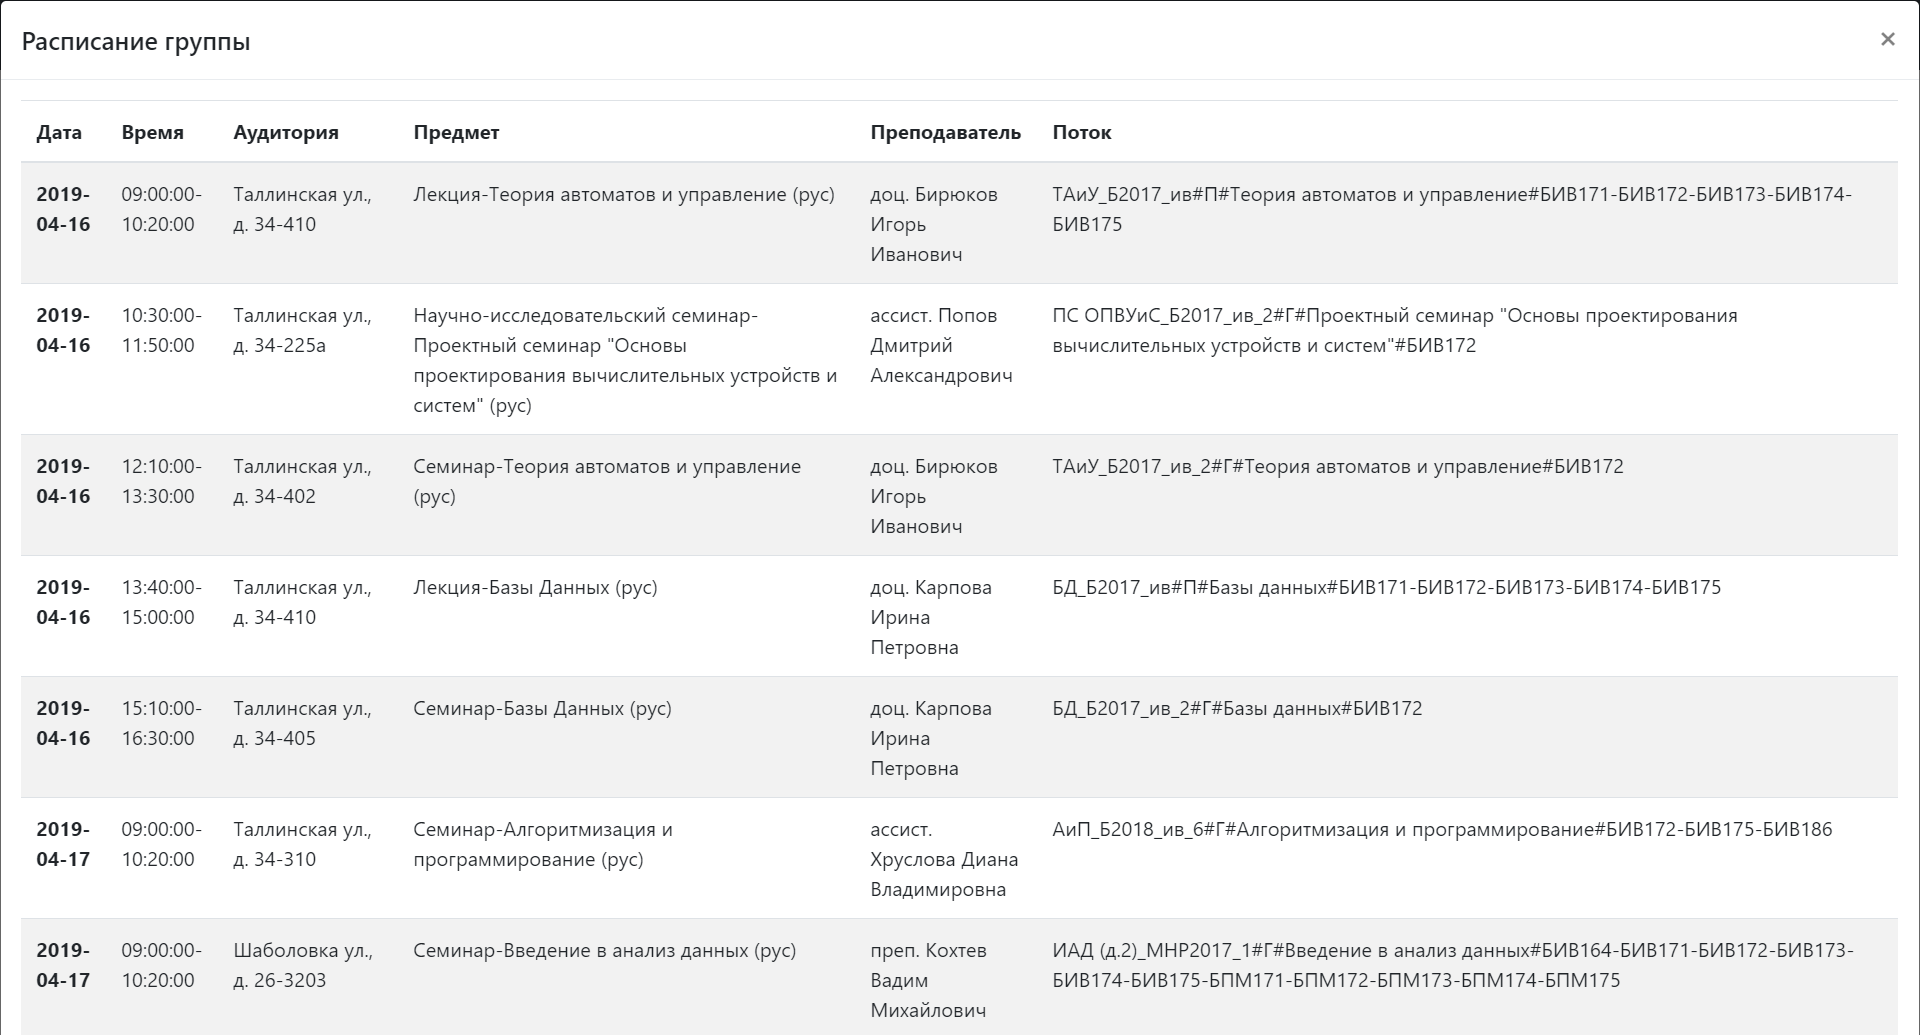
\includegraphics[width=\linewidth]{image/ui_scheduler}
	\caption{Форма просмотра расписание группы}
	\label{img:ui_scheduler}
\end{figure}

На странице поиска групп, которая находится на \url{/ruz/findGroup.php} можно найти интересующие записи с помощью формы ввода названия группы, подходящие варианты будут отображены на экране (Рис. \ref{img:ui_search}) с возможностью сразу создать курс на основе данной группы (Рис. \ref{img:ui_newGroup}), однако для уже существующих групп такой возможности нет для обеспечения сохранения условий целостности системы.

\begin{figure}[H]
	\centering
	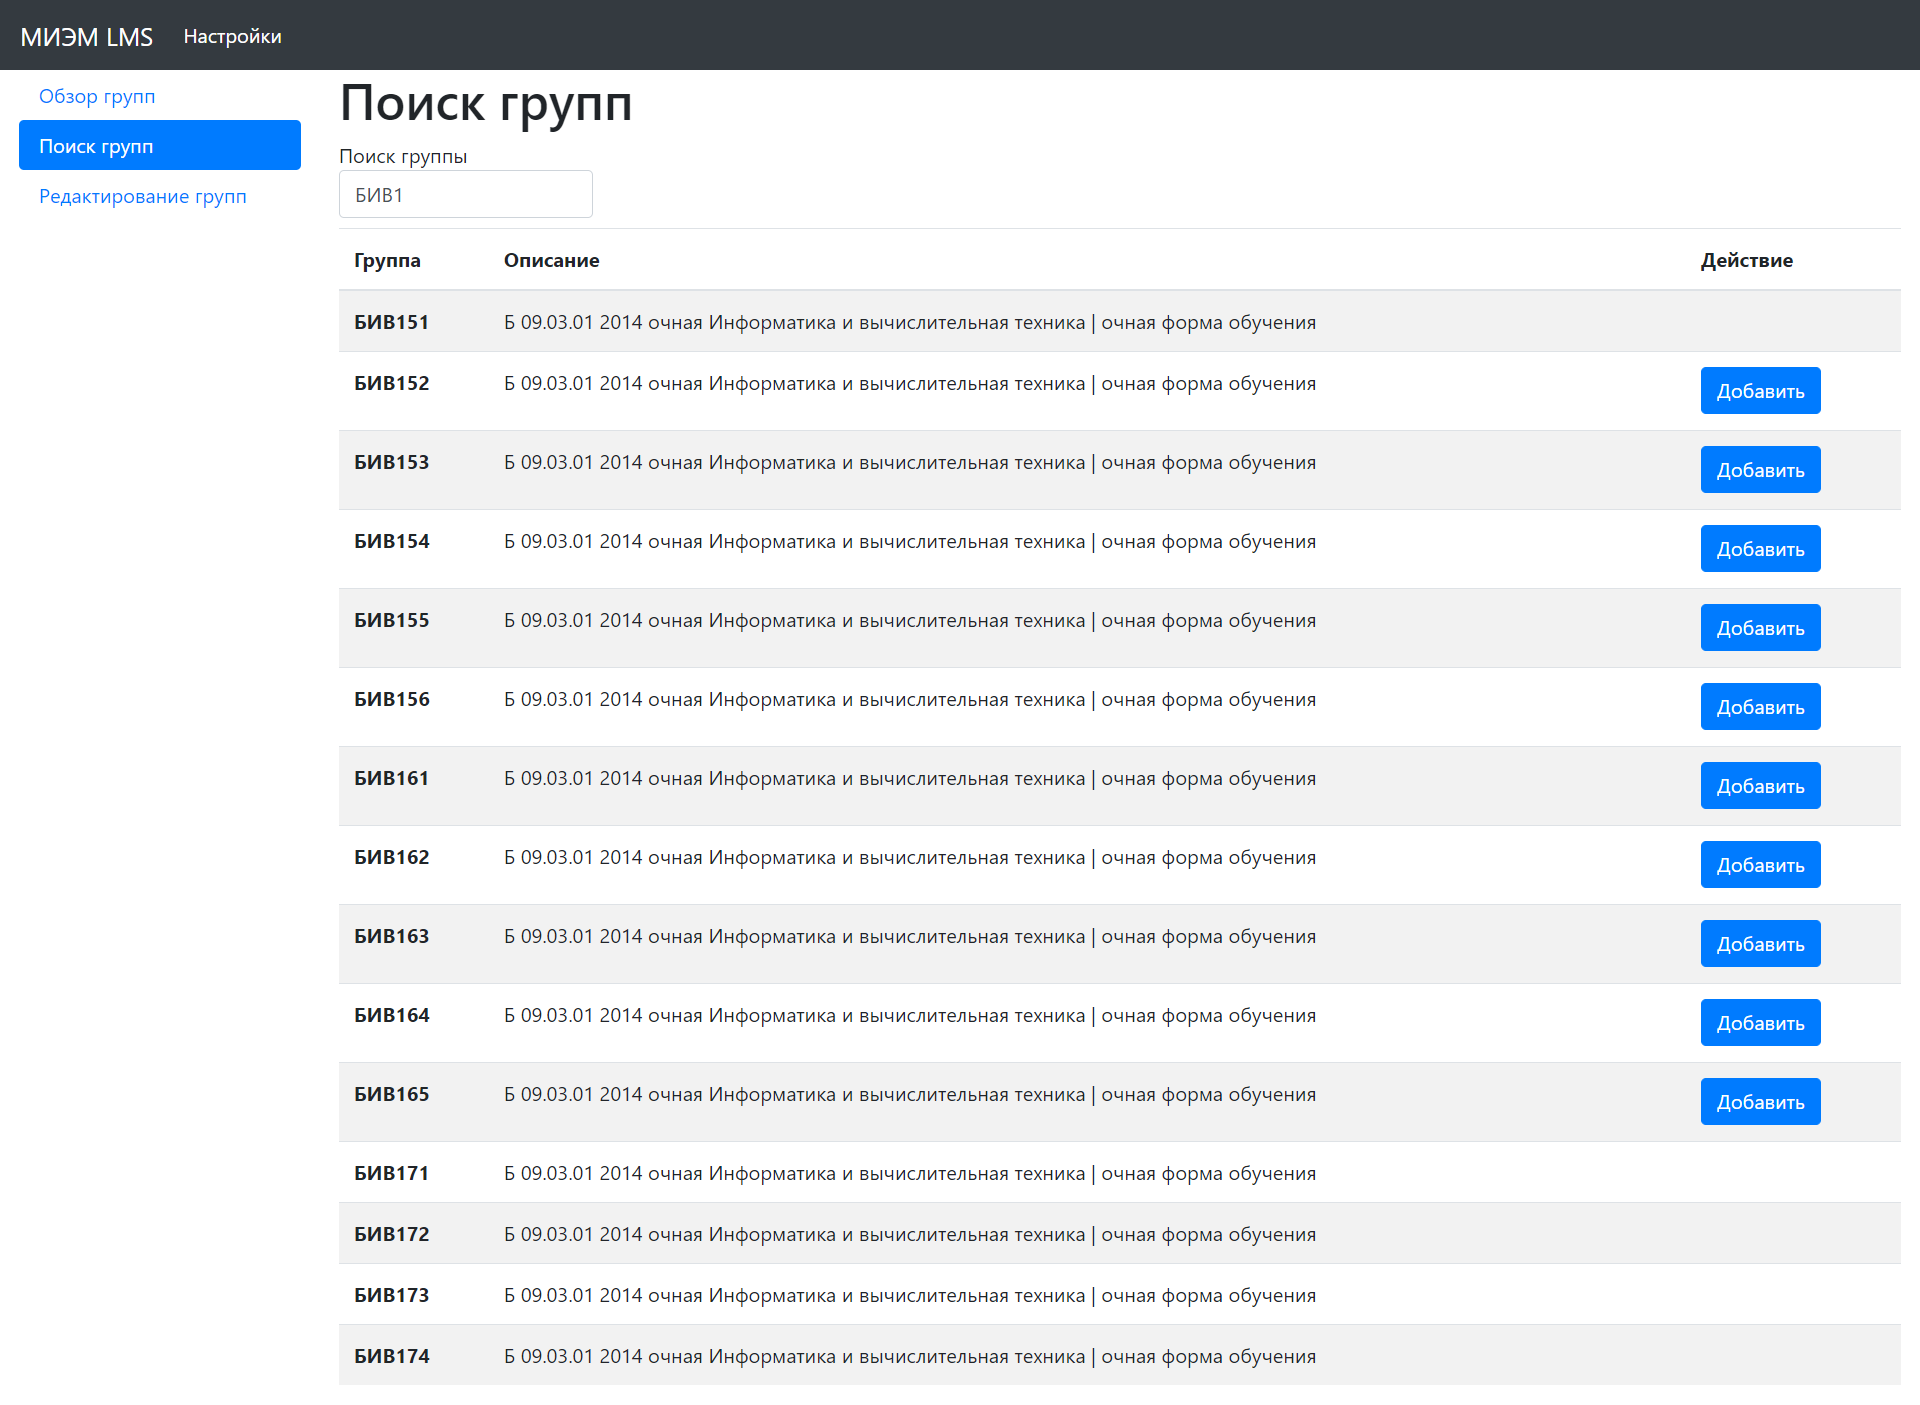
\includegraphics[width=\linewidth]{image/ui_search}
	\caption{Страница поиска группы}
	\label{img:ui_search}
\end{figure}
\begin{figure}[H]
	\centering
	
\includegraphics[width=\linewidth]{image/ui_newGroup}
	\caption{Форма создания курса}
	\label{img:ui_newGroup}
\end{figure}

Страница редактора группы (\url{/ruz/editGroup.php}) (Рис. \ref{img:ui_groupEditor}) позволят записать единичного пользователя (Рис. \ref{img:ui_newUser}) или перейти на страницу с возможностью загрузки нескольких пользователей одновременно.

\begin{figure}[H]
	\centering
	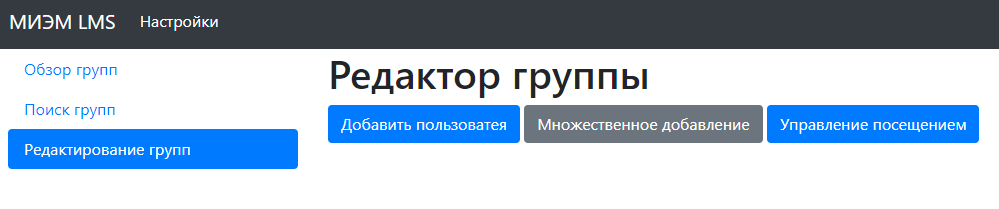
\includegraphics[width=\linewidth]{image/ui_groupEditor}
	\caption{Страница редактора группы }
	\label{img:ui_groupEditor}
\end{figure}
\begin{figure}[H]
	\centering
	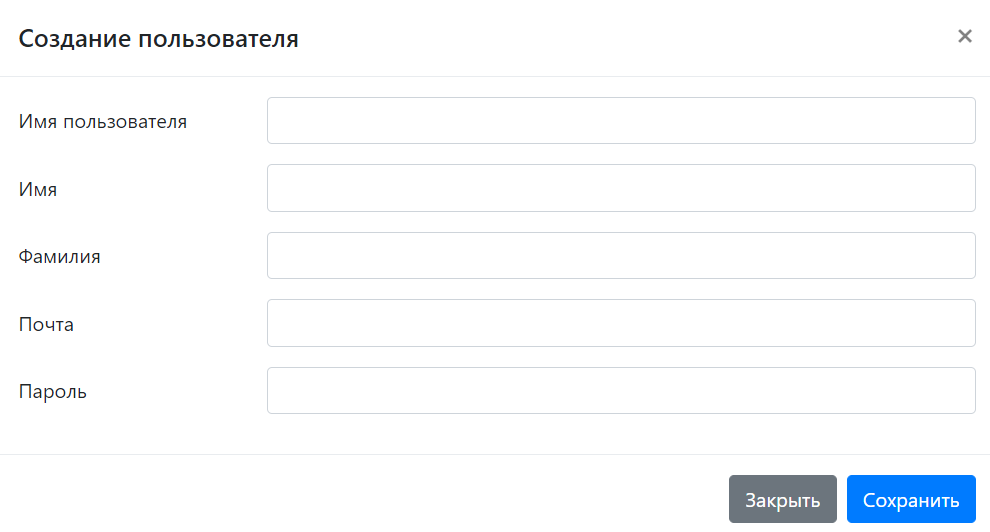
\includegraphics[width=\linewidth]{image/ui_newUser}
	\caption{Форма записи пользователя}
	\label{img:ui_newUser}
\end{figure}

Для служебный действий или автоматизации с другими сервисами предусмотрен API по адресу \url{/ruz/api/*}.
Доступные действия:
\begin{itemize}
	\item \url{/ruz/api/attachUser.php} -- записать пользователя на курс
	\item \url{/ruz/api/createGroup.php} -- создать группу
	\item \url{/ruz/api/createUser.php} -- создать пользователя
	\item \url{/ruz/api/findGroup.php} -- найти группу в РУЗе
	\item \url{/ruz/api/getGroup.php} -- получить группы
	\item \url{/ruz/api/getUser.php} -- получить пользователей
	\item \url{/ruz/api/ruzDisplay.php} -- отобразить расписание 
	\item \url{/ruz/api/ruzFetch.php} -- получить свежее расписание с РУЗа (доступно так же в CLI режиме, автоматически выполняется через cron)
\end{itemize}
% Анализ результатов

% Подтверждение актуальности

% Выводы и заключение
\subsection{Выводы по главе}

В данной главе были рассмотрены этапы реализации программной части работы.
Был показан список необходимого программного обеспечения, требуемого для корректной работы комплекса, порядок установки и настройки.
Кроме того, был показан пользовательский интерфейс и способ взаимодействия с ним, программный интерфейс и его функционал.
Так же в главе описаны возможности системы Moodle с установленными плагинами.
Была создана информационная система, которая решает задачи автоматизации учебного процесса.


% Конец Г4
% ==============================================================================
% Начало заключения

% Результаты

% Научная новизна и практическая значимость

% Личный вклад каждого соавтора работы, даже если автор 1

% Ваши выводы

% Предполагаемое применение полученных результатов

% Направление дальнейших исследований (перспективы дальнейшего развития работы)

% Конец заключения
% ==============================================================================
\end{document} % конец документа

